% !Mode:: "TeX:UTF-8"
% !TEX program  = xelatex

% \section{一些样例}

% \subsection{表格}

% \begin{table}[htb]
% % h-here,t-top,b-bottom,优先级依次下降
%     \begin{center}
%     % 居中
%         \caption{表格的标题应该放在上方}\label{table}
%         \begin{tabular}{lc} % 三线表不能有竖线,l-left,c-center,r-right
%             \toprule
%             %三线表-top 线
%             Example & Result \\
%             \midrule
%             %三线表-middle 线
%             Example1          & 0.25 \\
%             Example2          & 0.36 \\
%             \bottomrule
%             %三线表-底线
%         \end{tabular}
%     \end{center}
% \end{table}

% \subsection{参考文献}

% 参考文献如是\cite{Nicholas1998Handbook}。

\section{建模与控制}

\subsection{引言}
机器人建模与控制是机器人研究中最重要的话题之一。机器人的建模既是研究者所关心的状态量与输入量之间的关系(例如输入关节电机角度,与输出末端位姿之间的关系),也可以是研究者所关心的量之间的关系(例如末端的速度,与关节速度的关系)。实际上,考虑到自然界的许多过程广泛设计动态系统,即其系统模型通常以常微分方程或偏微分方程所描述,实际上机器人建模也是状态量自身现在与过去的关系。而对于机器人而言,实际上所有刚体机器人建模归根结底都可以表达为描述了机器人全部的微分方程,这里强调刚体是因为刚体机器人中状态数目是有限的,而软体机器人的状态甚至不是可数(countable)的,而从上述方程中,通过选取部分、抽象封装的方式,便可以获得需要研究的建模内容。具体而言,读者可能会反驳如何从刚体机器人的动力学模型中获得正向或者逆向的位置运动学,而笔者的论点是:将电机能够提供位置模式、速度模式这样具体的想法便已然是一种抽象与封装。对于电动机而言,其无法静态地、开环地、稳定地提供速度或者位置地输出,实际上其运动地一切根源均来自牛顿第三定律。因而,其输出扭矩到输入电流之间便有一种理想的映射,并以电动机转矩常数冠名。读者可能会继续反驳,在电动机内部,难道就是这样理想的映射?笔者则继续解释称,理想电动机内部如是,但实际电动机存在转子惯量和线圈电感,因而并不能认为是给定电流便理解输出相应扭矩的模型,自然会有同样的动态过程。而进一步的,电动机也并不理想,因而上述电流到扭矩之间的映射也不是持续可靠,甚至在其工作范围内也不成立。因此,考虑到误差的可接受度,笔者也对其进行了一定的简化。具体而言电动机的转子和线圈对其输出扭矩的影响,分别以机械时间常数与电气时间常数称呼,来自于其动力学方程,一个一阶常微分方程中的时间常数。考虑到时间常数甚小,因此对机器人的影响较小,因而将之忽略,从而简化机器人动力学模型。如果归根结底地将电机的更上一级的电机控制器内部的动态过程也考虑进去,整个系统会变为混合系统,且更为复杂——因为在电机控制器中,不仅存在连续的动态系统,也存在离散的动态系统,即使是用于处理的逻辑芯片与存储数据的内存,其本质上与人类在发明他们时制造的三极管和电容无二异,芯片的设计也需要考虑流水线、寄存器的读取速度与时钟周期,并伴随着随机性的电压与校验错误的影响。因此,如果这些内容不加以抽象,整个动力学将会过于复杂。但是,抽象的程度并无确定性的答案,例如电机可抽象为电流环,也可抽象为速度环,还可抽象为位置环,这些都将取决于具体的情况所定。当然,对于抽象过的内容,一般也会有其性能表征,例如电机的机械时间常数与电气时间常数便是其性能表征的体现;而对于电机控制器和处理器,其能够运行的频率和延迟,也同样是性能表征的一部分。我们也可以用以这测试驱动开发(TDD,Test driven development)的方式理解,之所以要解开位置和速度的封装,有的时候时是因为单纯的位置或者速度控制隐藏了太多的内容,无法达到预期的表现,或者是现在的技术已经足以面对更加复杂的系统,对更加复杂的系统进行建模,则对其了解更多,控制效果更好。另一方面,电动机、电机控制器也不可能根据机器人科学家的想法进行随心所欲的定制,因此更多时候需要将他们假设成一个黑箱子(Oracle),面向可以获得的信息建模。这时候就有通过控制位置或者速度的方式实现力控了,读者不妨想象如下的过程:对于理想的机器人电机和控制器而言,如果规定机械臂需要执行的运动轨迹,则可以通过动力学方程反推出电机的扭矩;但如果使用理想的电机和控制器用位置逆解的方式跟踪,则此时检查电机的扭矩,便毫无疑问地会发现二者一致。在这里,笔者愿称之为孪生或者对偶,其实际上是同一件事情的两面。因此回到一开始读者的提问,便是如何从动力学模型中提取出运动学模型?在这里终于可以给出解答:利用动力学模型,反算出研究者关心的变量分别与动力学模型中所有变量的关系,然后进行化简即可。笔者在这里需要提及广义的方程组求解:对于线性方程组,朴素的解法是根据矩阵本身的特性求解,而或者是使用广义逆等方式求解,但其都可以划归为寻求满足方程约束的解与优化变量之间距离。根据距离函数(范数)的定义不同,如果是欧几里得范数,则可以被认为是一种二次规划(QP)问题。在这一段落的尾声,笔者必须指出:可以从动力学模型中获取运动学模型并不代表我们将这么做,实际上更多时候或许是不可能的,实际上本章剩余的部分也将遵循一种位置运动学-速度位置学-动力学的范式。这里想表达的是,运动学模型与动力学模型之间是并不割裂的,而是一种推广的关联关系,或者可以成为动力学模型“蕴含”(Entail)了运动学模型。

回到具体的轮腿机器人上,其一般被简化为小车-倒立摆(Cart-Pole)模型,是一种典型的欠驱动机器人,因此即使是简单的静态平衡也涉及相对多的控制算法。机器人在CAD软件设计之后,可以获得准确的尺寸和粗略的质量、质心位置和转动惯量参数,而由于仿真的自定特性,CAD模型可以直接用于构建仿真模型。但是实物原型机出于各种原因(部分零部件没有质量、质心数据),仍然需要进行单独的参数辨识。一般而言,参数辨识可以离线完成,也可以在线使用观测器实现。对于实现简单的平衡控制,通过离线测定重心位置的方式就有相对不错的效果。在线使用观测器则涉及了非线性的系统辨识,一般采用扩展卡尔曼滤波实现(EKF)。仿真模型可以认为是实物原型机的数字孪生。
在拥有必要的参数后,可以通过对机器人建模的方式研究其系统,一般而言,机器人拥有运动学和动力学模型,而控制器则通过这些模型和实际情况去设计。当机器人需要实现变高度时,由于胯部和膝盖电机都工作在位置模式,所以一般是使用位置运动学模型进行工作空间到关节空间的转换,然后使用位置模式去控制;而但机器人需要实现简单的PID平衡时,则需要根据机器人实现测定的重心位置,或者每个杆件的重心位置通过机器人构型计算出来的结果,去跟踪重心与竖直线的偏差,以实现控制;如果是使用LQR进行空间的轨迹跟踪,则需要根据动力学模型线性化为状态空间方程,并选取选哟控制的状态量,然后根据Q与R惩罚矩阵设计对应的状态变量增益K。其中涉及到的质心位置,可以通过实现测定和根据构型计算,也可以通过EKF进行观测,在线调整,例如在机器人被加载负载时,则只能通过上述在线调整方法。

\subsection{建模}
一般而言,运动学包括位置运动学正逆解和微分/速度运动学\cite{corke2011robotics}\cite{lynch2017modern}(雅可比运动学)。位置运动学正解是:给定驱动器的各关节角度,计算末端或指定刚体的位姿(pose),这在计算雅可比矩阵和动力学时有重要作用。
速度运动学,或雅可比运动学,是关节空间的速度和末端或指定刚体速度的映射关系,且是双射。雅可比矩阵可以运用在微分逆运动学控制中;由于空间力和速度的对偶关系,根据虚功原理,可以得出雅可比矩阵的转置同样是相同末端或指定刚体受到的合外力到关节空间扭矩的映射,称之为力雅可比矩阵。
对于任何机器人,欧拉-拉格朗日法都可以用于分析动力学,从而建立状态方程。但是这种方法对于符号计算和技巧要求较高,并不适合一些基于动力学的控制方法,因此对于固定基座的串联机器人,一般采用递归牛顿欧拉法,虽然这并不适用于轮腿机器人,但是可以首先假设轮子与地面关系,然后使用IMU的读书带入线性方程,从而解算出机器人扭矩和运动状态的关系。
基于动力学控制的优点显而易见:力是运动改变的原因,而电机无法在外界负载变换的情况下,对位置和速度进行高频的良好跟踪。电机负载越大,上述跟踪越差。而电机力控则可以实现高频跟踪,并且性能与负载无关。速度和位置的性能差的原因,来自于电机内部的控制器是无法接受外界信息,尤其是前馈信息的,因此很难在任何负载及负载变化下达到最优。而动力学控制正是根据需要跟踪的轨迹和机器人动力学模型反算出电机的前馈力矩,使得电机的反馈力矩是线性的,从而可以达到一致的较好效果。

\subsubsection{运动学模型}

本子节中,运动学模型既包括机器人本身部件之间的运动学模型,也包括机器人作为移动机器人的运动学模型。

关于机器人杆件之间的运动学模型,为了简化模型,目前仅对轮腿机器人的建立简单的矢状面(如图\ref{fig:sec2-3lim})运动学模型,考虑到轮子与地面并不固连且持续旋转,且认为机器人构型不会经常改变,因此选取z轴与小腿方向重合的坐标系B,根据膝关节和胯关节电机的角度以及对应杆件质量、长度,可以计算出质心位置和IMU位置,从而计算出IMU测量的俯仰角与实际上质心与铅垂线的偏差角度,从而利用此角度设计PID或LQR控制器。如图\ref{fig:sec4-frame}所示:

\begin{figure}
  \centering
  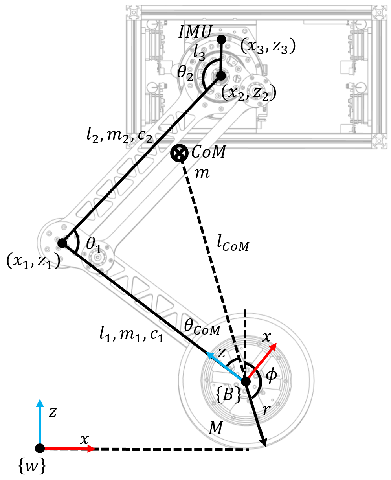
\includegraphics[width=0.5\linewidth]{figures/Sec4/frame.png}
  \caption{
  矢状面建模及相关物理量符号定义示意图。
  }
  \label{fig:sec4-frame}
   \vspace{6pt}
\end{figure}

其中轮腿变高度与电机角度的关系和上述角度偏差关系如下:
$\{w\}$为世界系, 而$\{B\}$是中心和轮子中心重合,但$z$方向总是指向膝关节的座标系。$\phi$轮子自从初始位置开始旋转过的角度,因而$x_B = \phi r,\ y_B = r$.小腿和大腿的质量、长度和质心位置分别是$(l_1,m_1,c_1),\ (l_2,m_2,c_2)$,这些数据都可以从CAD模型中获得。$\theta_1,\ \theta_2$则由膝关节和跨关节的电机决定,且如果机器人完全直立站起,$\theta_1 = \theta_2 = \pi$.机器人躯干的质心被认为是与胯关节的中心重合,而IMU安装在距离中心$l_3$的位置。于是我们可以计算在$\{B\}$系下的质心位置:
\begin{equation}
\begin{bmatrix}
    x_{CoM} \\
    z_{CoM}
\end{bmatrix}
=
\frac{
\sum_i^{} m_i
\begin{bmatrix}
    x_{c_i} \\
    z_{c_i}
\end{bmatrix}
}{\sum_i^{} m_i}
\label{eq:com_calc}
\end{equation}

类似的,在$\{B\}$系下的每个点的坐标可以用如下的公式计算出来:
\begin{equation}
\begin{bmatrix}
    x_{c_1} \\
    z_{c_1}
\end{bmatrix}
=
\begin{bmatrix}
    0 \\
    c_1
\end{bmatrix}
    \label{eq:kine_c1}
\end{equation}

\begin{equation}
    \begin{bmatrix}
        x_{c_2} \\
        z_{c_2}
    \end{bmatrix}
    =
    \begin{bmatrix}
        c_2 sin\theta_1 \\
        l_1 - c_2 cos\theta_1
    \end{bmatrix}
    \label{eq:kine_c2}
\end{equation}

\begin{equation}
    \begin{bmatrix}
        x_{c_3} \\
        z_{c_3}
    \end{bmatrix}
    =
    \begin{bmatrix}
        l_2 sin\theta_1 \\
        l_1 - c_2 cos\theta_1
    \end{bmatrix}
    \label{eq:kine_c3}
\end{equation}

从根据公式\ref{eq:com_calc},公式\ref{eq:kine_c1},公式\ref{eq:kine_c2} 和公式\ref{eq:kine_c3}中,我们可以计算${B}$系下的等效质心位置。而要计算质心与竖直线之间的夹角,我们需要结合质心位置与IMU测量数据。IMU在${B}$系下的位置是:

\begin{equation}
    \begin{bmatrix}
        x_3 \\
        z_3
    \end{bmatrix}
    =
    \begin{bmatrix}
        l_2 sin\theta_1 - l_3 sin(\theta_1 - \theta_2) \\
        l_1 - l_2 cos\theta_1 + l_3 cos(\theta_1 - \theta_2)
    \end{bmatrix}
    \label{eq:kine_3}
\end{equation}

那么IMU和质心之间的夹角就是

\begin{equation}
    \theta_{CoM} = atan2(z_3 - z_{CoM}, x_3-x_{CoM})
    \label{eq:theta_com}
\end{equation}

由于IMU直接测量了其与竖直线之间的夹角$\theta_{IMU}$,所以质心与竖直线之间的夹角是:

\begin{equation}
    \theta = \theta_{IMU} + \theta_{CoM}
    \label{eq:theta_calc}
\end{equation}

\begin{figure}[h!]
  \centering
  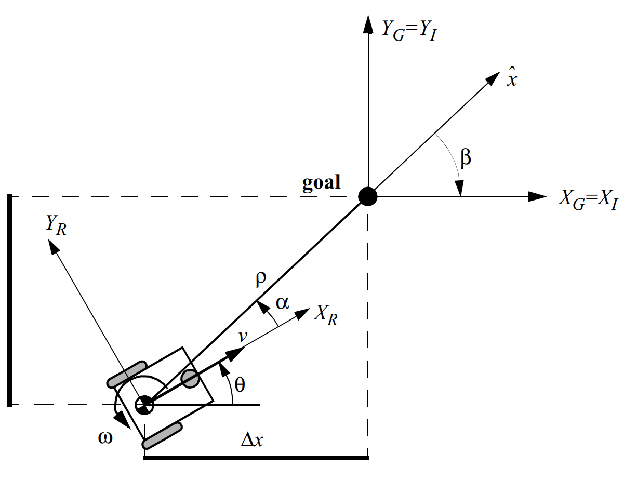
\includegraphics[width=0.6\linewidth]{figures/Sec4/kingoal.png}
  \caption{
  移动机器人动力学示意图\cite{siegwart2011introduction}。
  }
  \label{fig:sec4-kingoal}
   \vspace{6pt}
\end{figure}

而考虑移动机器人动力学时,本轮腿机器人由两个差速转向的轮子控制运动,具体如图\ref{fig:sec4-kingoal}所示。取$[x,y,\theta]^T$为机器人的状态变量,则机器人的状态与其线速度、角速度的关系如公式\ref{eq:stalinang}所示。

\begin{equation}
    \begin{bmatrix}
        \dot{x} \\ \dot{y} \\ \dot{\theta}
    \end{bmatrix} = 
    \begin{bmatrix}
        cos \theta & 0 \\ sin \theta & 0 \\ 0 & 1
    \end{bmatrix}
    \begin{bmatrix}
        v \\ \omega
    \end{bmatrix}
    \label{eq:stalinang}
\end{equation}

考虑到后文中提到机器人需要进行轨迹跟踪,因此在给定如图\ref{fig:sec4-kingoal}中的目标点后,我们需要计算其中的参数$\alpha$、$\beta$和$\rho$。在这里将采用极坐标转换如公式\ref{eq:cat2rho}所述,变换为如公式所述的形式,于是可以得到机器人与目标点之间的关系,而利用这个关系可以作为反馈控制,以达到给定的目标点。
\begin{equation}
    \begin{aligned}
      \rho & = \sqrt{\Delta x^2 + \Delta y^2} \\
      \alpha & = -\theta + atan2(\Delta y, \Delta x) \\
      \beta & = -\theta -\alpha 
    \end{aligned}
    \label{eq:cat2rho}
\end{equation}

\begin{equation}
    \begin{bmatrix}
        \dot{\rho} \\ \dot{\alpha} \\ \dot{\beta}
    \end{bmatrix} = 
    \begin{bmatrix}
        -cos\alpha & 0 \\ \frac{sin \alpha}{\rho} & -1 \\ -\frac{sin\alpha}{\rho} & 0
    \end{bmatrix}
    \begin{bmatrix}
        v \\ \omega
    \end{bmatrix}
\end{equation}

而对于机器人的速度$[v,\omega]^T$与机器人轮速之间的关系,假设机器人轮间距为$2d$,则不难推出其关系如公式所示。
\begin{equation}
    \begin{bmatrix}
        v \\ \omega
    \end{bmatrix} = 
    \begin{bmatrix}
        \frac{1}{2} & \frac{1}{2} \\ \frac{1}{d} & -\frac{1}{d}
    \end{bmatrix}
    \begin{bmatrix}
        v_1 \\ v_2
    \end{bmatrix}
    \label{eq:naveq}
\end{equation}

\subsubsection{动力学模型}
正如引言中所述,力是运动改变的原因。对于固定底座的机械臂而言,即使不考量动力学模型,依然可以通过位置控制或者微分逆运动学进行速度控制来实现轨迹跟踪。虽然在PID平衡中,动力学也可以不考虑,但是其进行矢状面轨迹跟踪是依靠对轮子编码器的加权和饱和作为偏差输入到控制器中,这种控制方式虽然能实现效果,但需要仔细调整权重和饱和;而一般而言,对于轮腿机器人来说,如果有动力学模型则可以获知整个系统的向量场,从而使用LQR的方式收敛到任意的向量场中可控的一点。
考虑到轮腿机器人的膝关节和胯关节工作在位置模式下,因此并不考虑腿部的动力学,而轮腿的轮子转动惯量先对于系统其他部分对动力学的影响较小,因此可以忽略,则轮腿可以简化成小车-倒立摆模型。这里倒立摆并不视为一个质点,因此需要计算转动惯量。其中一种方式是利用CAD模型给出的粗略的转动惯量矩阵,在坐标变换后相加,然后计算绕轮子中心轴的转动惯量。另一种方式是将每个杆件视为质点,然后利用平行轴定理计算转动惯量之后相加。由于整体的质心位置也需要使用机器人构型计算,因此在实际控制中,采用的是后一种方式。

为了更简便的控制,我们对膝关节和胯关节电机采取静力学假设。如公式\ref{eq:com_calc}所示,质心在${B}$系下的位置,和整个机器人在其中的转动惯量都是与膝盖和胯部电机有关的函数。为了进一步简化,我们假设所有杆件都是质点,这样可以根据每个杆件的质心计算公式\ref{eq:kine_c1},公式\ref{eq:kine_c2}和公式\ref{eq:kine_c3},所有杆件(除了轮子)的转动惯量式:
\begin{equation}
    I = 2m_1 (x_{c_1}^2+z_{c_1}^2) + 2m_2 (x_{c_1}^2+z_{c_1}^2) + m_3 (x_{c_1}^2+z_{c_1}^2)
    \label{eq:inertia}
\end{equation}

\begin{figure}
  \centering
  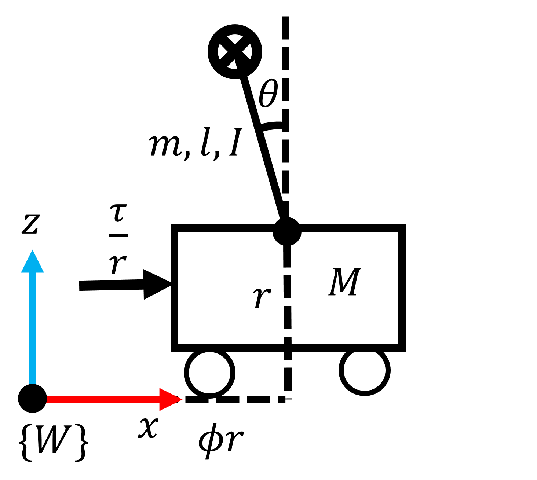
\includegraphics[width=0.4\linewidth]{figures/Sec4/2dsimple.png}
  \caption{
  矢状面动力学模型符号定义示意及小车-倒立摆模型建图。
  }
  \label{fig:sec4-2dsimple}
   \vspace{6pt}
\end{figure}

由于轮子的转动惯量较小,相对于整个机器人,其影响机器人的动力学较少,因此机器人可以简化成一个小车-倒立摆模型。我们定义$f = \frac{\tau}{r}$以及$x = \phi r$,这样我们使用欧拉-拉格朗日公式就可以计算出动力学模型。在这里,我们首先考虑矢状面的动力学模型,然后考虑空间中的动力学模型。其中机器人的矢状面定义如图\ref{fig:sec2-3lim},而其简图如xxx所示。除了欧拉-拉格朗日公式,还可以使用另外两种分析方式,这里也将详细展开。欧拉-拉个朗日法聚焦于能量视角,其中系统的广义位置、广义速度分别为$q$,$\dot{q}$,对应的广义力为$   \tau$,针对广义速度可计算出系统的整体的动能$T$与势能$V$,并定义$L=T-V$则可以用公式\ref{eq:eu-la}求出广义力:

\begin{equation}
    \tau = \frac{\partial L}{\partial \dot{q}} - \frac{\partial L}{\partial q}
    \label{eq:eu-la}
\end{equation}

对于本轮腿机器人,上述动能为小车部分与倒立摆的动能之和:

\begin{equation}
    T=\frac{1}{2}(M+m)\dot{x}^2 + m\dot{x} \dot{\theta} l cos \theta + \frac{1}{2} m l^2 \dot{\theta}^2
    \label{eq:la-T}
\end{equation}

而势能则只与倒立摆的角度,相应的质心高度,有关:

\begin{equation}
    U=-mglcos \theta
    \label{eq:la-V}
\end{equation}

通过式\ref{eq:eu-la},式\ref{eq:la-T},式\ref{eq:la-V},可以计算系统的动力学方程如下:

\begin{equation}
    (M+m)\ddot{x} - ml\ddot{\theta}cos\theta -ml\dot{\theta}^2 sin\theta = f
    \label{eq:motion1}
\end{equation}

\begin{equation}
    ml^2\ddot{\theta} + mgl sin\theta = ml\ddot{x}cos\theta
    \label{eq:motion2}
\end{equation}

\begin{figure}
  \centering
  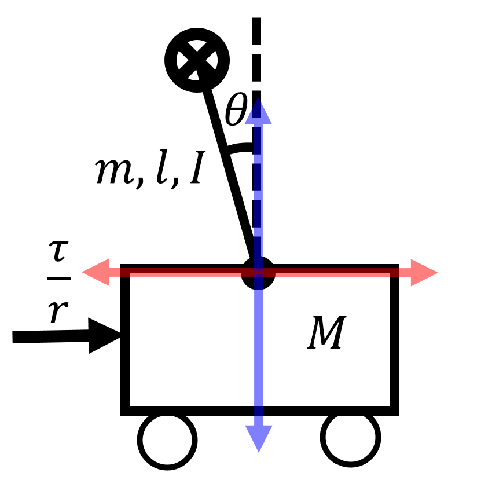
\includegraphics[width=0.4\linewidth]{figures/Sec4/2d2.png}
  \caption{
  矢状面受力分析图(F.B.D.)符号定义。
  }
  \label{fig:sec4-2d2}
   \vspace{6pt}
\end{figure}

接下来讨论另一种简单的基于分析的方法,以及它的牛顿-欧拉法的变种,最后使用这种方法推广到三位空间中的线性倒立摆模型。首先我们考虑朴素的受力分析方法,具体来说,首先分析每个被隔离的杆件。具体各种力的定义如图\ref{fig:sec4-2d2}所示,关于小车的受力如公式\ref{eq:cart-f}所示。
\begin{equation}
    M\ddot{x} = F - N
    \label{eq:cart-f}
\end{equation}
而关于铰链处的力$N$的表的是则如公式\ref{eq:cart-n}所示。
\begin{equation}
    N = m\ddot{x} + ml\ddot{\theta}cos \theta - ml\dot{\theta}sin \theta
    \label{eq:cart-n}
\end{equation}
接着沿着倒立摆方向的受力如公式\ref{eq:cpf}所示。
\begin{equation}
    Psin\theta N cos\theta - mgsin \theta = ml\ddot{\theta} + m\ddot{x} cos\theta
    \label{eq:cpf}
\end{equation}
通过转矩关系(公式\ref{eq:pnrel})消去$P$和$N$以获得最终的结果。

\begin{equation}
    -Plsin\theta - Nlcos\theta = I\ddot{\theta}
    \label{eq:pnrel}
\end{equation}

最终得到与公式\ref{eq:motion1}和公式\ref{eq:motion2}相同的结果。

在这里,我们可以总结出牛顿欧拉法的具体使用方式:首先确定所有杆件,并据此定义状态变量。每个刚体具有6个自由度,定义杆件数$\times$6的状态变量之后,首先寻找杆件自身的约束,如杆件固定在地面上,或杆件须沿指定轴旋转(相应的便是5维的约束力),然后寻找相关杆件之间的约束,大多数机器人关节都可以用极简易的方式定义,一些相对复杂的例如圆柱沿斜面无滑动的滚动也可以首先找到可能的运动空间,然后寻找该运动的对偶空间,其基便是约束力。接下来,针对每个杆件,将与之相关的力,包括电机的扭矩、约束力、重力和约束力。值得注意的是,惯性力、科氏力(Coriolis Force)和陀螺力(Centrifugal Force)并不考虑在内,这是因为牛顿欧拉方程\cite{featherstone2014rigid}(如公式\ref{eq:newtoneul})已经将他们考虑在内了。

\begin{equation}
    \mathcal{F} = \mathcal{I}\mathcal{A} + \mathcal{V}\times^* \mathcal{I} \mathcal{A} + \mathcal{J}^T\mathcal{F}_{ext}
    \label{eq:newtoneul}
\end{equation}

在上述公式中,所有杆件必须换算在同一坐标系下。其中$\mathcal{I}$是空间转动惯量,$\mathcal{V}$是空间速度,$\mathcal{A}$是空间加速度,$\mathcal{J}$是接触力的雅可比矩阵,$\mathcal{F}$是空间力,$\times^*$是定义在空间速度上的叉乘,是一个确定的线性变换,甚至可以认为是同构,具体而言就是将空间速度这一6维向量转换成了一个6$\times$6的矩阵形式。上述讨论产生的方程组在有时出于“未知数过多,方程太少”的原因会有多解,例如轮腿机器人这一欠驱动系统,轮子与地面之间的接触无法检测,因此相应的甚至无法建立相应的方程。此时考虑轮腿上的传感器IMU,可以根据轮腿的其他关节的运动状态计算出轮子与地面之间的接触模型。

\begin{figure}
  \centering
  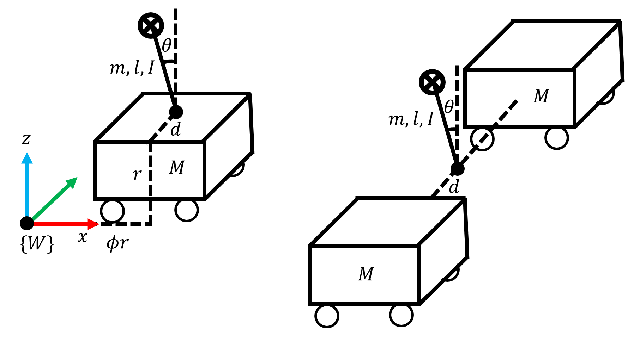
\includegraphics[width=0.45\linewidth]{figures/Sec4/3dsimple.png}
  \caption{
  空间的动力学模型符号定义示意及小车-倒立摆模型建图。其中左图是是空间中的小车-倒立摆模型的示意图,右图则是进一步简化后,将左右轮分别视为两个小车,然后研究其上倒立摆的模型。
  }
  \label{fig:sec4-3dsimple}
   \vspace{6pt}
\end{figure}

对上述过程进行简化,接下来将推导空间的动力学模型。在这里依然采用小车-倒立摆模型,但是小车可以在二维平面上运动,如图\ref{fig:sec4-3dsimple}所示。其中考虑到轮子只能提供单自由度的转动,因此将其使用非完整约束如等式\ref{eq:3d-noh}所示。更加直观的说,每个轮子的速度只能与当前轮子的方向相同。

\begin{equation}
    \frac{\dot{y}}{\dot{x}} = tan \theta
    \label{eq:3d-noh}
\end{equation}

为简化计算,将两个轮子中间与倒立摆铰链连接的部分视为没有质量的物体,于是其位姿便于两个轮子的位置有如同等式\ref{eq:mid-pos}的关系。

\begin{equation}
    \begin{bmatrix}
        x \\
        y \\
        \theta 
    \end{bmatrix} = 
    \begin{bmatrix}
        \frac{x_1+x_2}{2} \\
        \frac{y_1+y_2}{2} \\
        atan2(y_2-y_1, x_2-x_1)
    \end{bmatrix}
    \label{eq:mid-pos}
\end{equation}

在此基础上,考虑二维小车-倒立摆模型,但是其中需要加上小车自转产生的角速度产生的陀螺力,使得公式\ref{eq:motion1}需要被修改为公式\ref{eq:motion3}。

\begin{equation}
    (M+m)\ddot{x} - ml\ddot{\theta}cos\theta - ml\dot{\theta}^2 sin\theta + \omega^2 lsin\theta cos\theta = f
    \label{eq:motion3}
\end{equation}

然后使用公式\ref{eq:mid-pos}反解出左右轮与中心点的关系并带入公式\ref{eq:motion1}和\ref{eq:motion3}中,即可得到机器人的三维空间中的动力学方程。

\subsubsection{状态空间方程}
一般而言,根据状态变量的选取,通过对动力学模型进行变换即可得到状态空间方程。这里令$u = f$,并取$[x,\dot{x}, \theta, \dot{\theta}]^T$作为状态变量,我们可以根据上述动力学模型(公式\ref{eq:motion1}和\ref{eq:motion2})获得矢状面的连续时间的状态空间方程:
\begin{equation}
    \begin{bmatrix}
        \dot{x} \\
        \ddot{x} \\
        \dot{\theta} \\
        \ddot{\theta}
    \end{bmatrix}
    =
    \begin{bmatrix}
        0 & 1 & 0 & 0 \\
        0 & 0 & \frac{m^2gl^2}{I(M+m)+MmI^2} & 0 \\
        0 & 0 & 0 & 1 \\
        0 & 0 & \frac{mgl(M+m)}{I(M+m)+MmI^2} & 0
    \end{bmatrix}
    \begin{bmatrix}
        x \\
        \dot{x} \\
        \theta \\
        \dot{\theta}
    \end{bmatrix}
    +
    \begin{bmatrix}
        0 \\
        \frac{I+ml^2}{I(M+m)+Mml^2} \\
        0 \\
        \frac{ml}{I(M+m)+Mml^2}
    \end{bmatrix}
    u
\end{equation}

如之前的章节所述,所有的状态变量,都可以通过IMU和轮子编码器读到。考虑到主控制器的选型与编程方式,这里需要对连续时间系统进行离散化。对于如公式\ref{eq:cl-sys}所示的连续时间系统,其离散化后如公式\ref{eq:dl-sys}所示。

\begin{equation}
    \begin{aligned}
    \dot{x} & = Ax + Bu \\
    y & = Cx + du
    \end{aligned}
    \label{eq:cl-sys}
\end{equation}

\begin{equation}
    \begin{aligned}
    x_{k+1} & = A_d x_k + B_d u_k \\
    y_k & = C_d x_k + D_d u_k \\ 
    A_d & = A + I \Delta t A \\
    B_d & = B \Delta t \\
    C_d & = C \\
    D_d & = D 
    \end{aligned}
    \label{eq:dl-sys}
\end{equation}

\subsection{控制}

\subsubsection{PID轨迹跟踪}
PID是一种广泛在工业界采用的控制其。其中缩写PID所代表的意思分别是比例、积分与微分。其具体控制原理的示意图如图\ref{fig:sec4-pidgram}所示,反馈量会与目标值进差值,然后对插值乘以一个比例作为控制量,同时对差值进行微分,然后在乘以一个比例叠加到刚刚的控制量上,最后对差值进行积分,乘以一个比例后在叠加至刚刚的控制量上,便成为了PID控制器。值得注意的是,其中的微分参数或者积分参数可以为0.

\begin{figure}[h!]
  \centering
  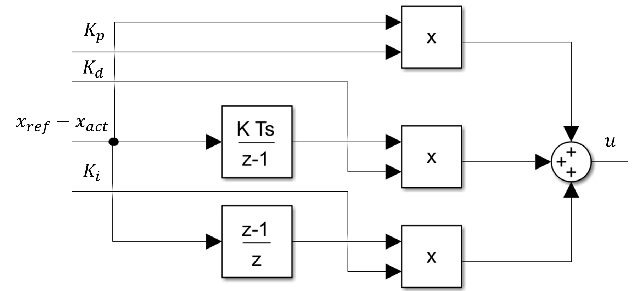
\includegraphics[width=0.75\linewidth]{figures/Sec4/pidgram.png}
  \caption{
  PID示意图
  }
  \label{fig:sec4-pidgram}
   \vspace{6pt}
\end{figure}

如前文所述,已知质心与竖直线夹角之后,可以建立PID控制器。但如果仅仅将期望位置加作为偏差,则控制器仅能保证机器人会位置在质心竖直向上的状态,但若质心测量稍有偏差,机器人就会维持一个恒定的加速度以维持平衡状态,而这显然是笔者所不希望看到的。此外,矢状面的轨迹跟踪的实现也与机器人在世界坐标系下的位置,也就是轮子编码器的具体角度息息相关,因此将轮子编码器当前值与目标值(目标位置)作为误差输入量之一输入PID控制器以实现矢状面的轨迹跟踪,如图\ref{fig:sec4-2dpid}所示。值得注意的是,考虑到机器人在失稳或者实验调试时轮子编码器可能会因为失败的平衡而记录错误的值,因此这里并不使用编码器上电值,而是平衡时且IMU读取线速度值极小时认为当前位置为原点。具体回到PID控制器,考虑到倾斜角度与机器人加速度相关,且当机器人质心接近于平衡状态时有$sin x \dot{=} x$,此时加速度实际上与倾斜角度成正比。因为可以使用此加速度控制机器人前进速度,而使用机器人前进速度控制机器人位置,因此可以将机器人的位置偏差作为输入量(系统观测量的偏差),将机器人的额外的倾斜角度作为输出控制量,叠加到上述PID控制器的角度偏差中。

\begin{figure}[h!]
  \centering
  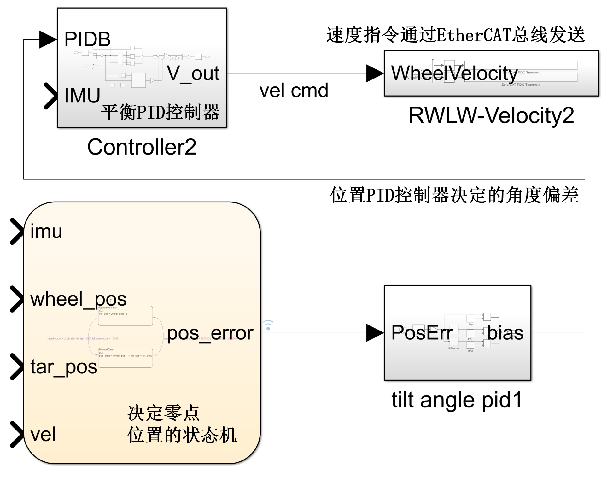
\includegraphics[width=0.75\linewidth]{figures/Sec4/2dpid.png}
  \caption{
  实际机器人矢状面PID控制器的示意图。
  }
  \label{fig:sec4-2dpid}
   \vspace{6pt}
\end{figure}

而转向则有差速转向开环实现,如图\ref{fig:sec4-3dpid}所示。当机器人接近平衡状态时,通过机器人角速度计算出每个轮子的速度差,从而叠加到轮子的指令速度上,再发送出去。当机器人不接近平衡状态时,此时机器人角速度会在质心产生陀螺力,从而影响机器人平衡状态,因此设有阈值,当机器人在平衡角度阈值内,才会执行转向指令。

\begin{figure}
  \centering
  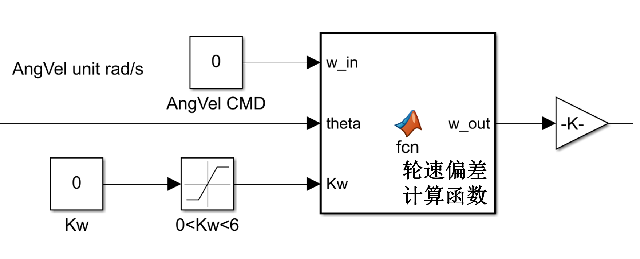
\includegraphics[width=0.8\linewidth]{figures/Sec4/3dpid.png}
  \caption{
  实际机器人3维轨迹追踪的差速转向控制器的示意图。其中输入量$Kw$是一个用于判定机器人倾角阈值的参数。
  }
  \label{fig:sec4-3dpid}
   \vspace{6pt}
\end{figure}

\subsubsection{LQR轨迹跟踪}
如前文所述,力是改变物体运动的原因。物体的运动可以通过物理定理,转化成微分方程,以方便研究。而已知物体运动的微分方程,也就知道可以在何种范围内修改物体的运动状态,以及以何种方式修改物体的运动状态。换句话说,在物体运动的状态空间中,控制是给出从当前状态到目标状态的路径(从路径可能随时间变化),将当前的全状态映射到可以控制的量上的函数,称之为控制率,如公式\ref{eq:ctrl_law}所示。
\begin{equation}
    u_{ctrl} = f(x_{state})
    \label{eq:ctrl_law}
\end{equation}
构建力与运动状态之间的关系并不是唯一可以用于控制的微分方程,但对于轮腿机器人这样欠驱动(underactuated)但可控(controllable)的系统,即使可以不使用力作为控制量,但使用力是最为简单与直观的。为简化控制,在得到状态空间方程如公式\ref{eq:dl-sys}所示后,便可以对可控的系统构建线性控制器。线性控制器并不是所有控制器中最优的(这取决于最优的定义),但却是最易于构建且简单的。其核心在于,给定线性常微分方程(组),通过对该微分方程进行参数化选择,修改该微分方程的审敛性。上述参数对状态量的速度(一阶导数)的影响是线性的,因此可以完美利用有理最简型(Rational Canonical Form)以修改常微分方程的极点(Pole)。虽然研究对象是离散空间,但是由于线性代数本质上是研究有限维向量空间上的线性算子(Linear Operator),收敛列等极限定理确保了其与连续时间空间中的常微分方程解相同,更何况皮卡存在唯一性定理(Picard's Existence and Uniqueness Theorem)的证明本身使用了皮卡序列(Picard's Sequuence),也就是将函数的极限视为函数列的极限。

然而,线性控制器中的零点的选择往往是没有强烈依据的,因而不合理的选择可能会使系统审敛过慢,抑或是超过系统控制变量可以输出的范围。因此,最用控制方法线性二次型规划器(Linear Quadratic Regulator, LQR)应运而生,其本质是通过对一个未来的时间片上的状态及输入量的惩罚(loss,又称cost),通过将控制问题转化成优化问题实现。对状态量的惩罚决定了系统为此响应的状态,而对输入量的惩罚决定了系统响应的幅度。尽管贝叶斯流派的机器学习科学家们可以将对线性回归的规范项(Regulator Item)成为之先验概率(Prior),但对于LQR来说并不可以。值得注意的是,线性回归往往是对于偏离模型的一种欧几里得模(Euclidean Norm)的惩罚,而LQR中的规范项Q和R,则分别是一种马哈拉诺比斯范数(Mahalanobis Norm)。实际上这里范数的选择,是为了方便求解LQR,将会在下文详细展开。值得注意的是,卡尔曼滤波器(Kalman Filter)也是一种线性回归,但是其并不是使用成批(Batched)的求解方式,而是一种在线(
online)的求解方式,可以认为数据点是逐个到来但要求任意时刻的结果。其核心类似于通项公式与递推公式的转换,也就是成批求解类似于通项的方式,给定初始值,给定所有输入;而递推公式则是仅给定上一个值和本次输入,在算法的时间和空间复杂度(Time and Space Complexity)上有其优势(在要求实时最优解的情况下)。

对于任意的递归约束、代价惩罚优化问题,都可以使用动态规划(Dynamic Planning)来求解,值得注意的是,LQR仅仅是其中一种情况。但动态规划的时间与空间复杂度过高,因此会利用LQR本身的特点递归求解,转化成线性问题。或者这样说更准确,并不是LQR选择了动态规划或其他求解方法,而是已经掌握的求解方法反向构造了LQR的形式;正如并不是线性控制器选择了极点放置的求解方法,而是已有的极点放置的求解方法选择了线性控制器。

另外,上述的LQR本身也有一定复杂性,因此我们再度简化,便为无穷时间片的LQR控制器,这里的简化实际上是一种粗略的近似,也即用LQR在平衡状态下的反馈增益代替趋向稳态时的反馈增益。

\begin{figure}[h!]
  \centering
  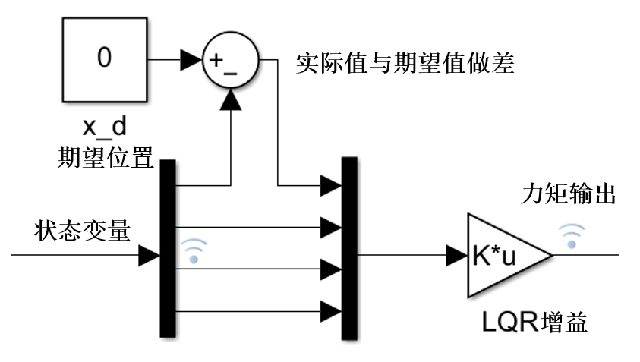
\includegraphics[width=0.65\linewidth]{figures/Sec4/lqrgram.png}
  \caption{
  实际仿真中,机器人采用的LQR控制器的示意图。
  }
  \label{fig:sec4-lqrgram}
   \vspace{6pt}
\end{figure}

为了实现鲁棒的平衡和轨迹跟踪,LQR\cite{li2012advanced}最优控制方法也被采用,并且用作和PID控制的对比。这里采用的式无穷水平线的固定反馈增益的LQR控制器,在给定状态变量惩罚矩阵$Q$和控制量惩罚矩阵$R$,最优的反馈控制增益$K$通过解如下的离散时间里卡蒂方程获得:
\begin{equation}
    P=A^TPA-(A^TPB)(R+B^TPB)^{-1}(B^TPA)+Q
    \label{eq:dare}
\end{equation}
我们已经获得了连续时间的状态空间方程,对其进行离散化之后,最优控制率可以用如下方式直接算出:
\begin{equation}
    K^* = (R+B^TPB)^{-1}B^TPA
    \label{eq:dare_sol}
\end{equation}

实际在仿真实验中,LQR控制器如图\ref{fig:sec4-lqrgram}所示。

\subsection{本章小结}

本章首先介绍了机器人的运动学和动力学模型,分别用在机器人的变高度控制和平衡控制,其中动力学模型进一步推导了状态空间方程。控制部分,首先介绍了简单的PID平衡及轨迹跟踪控制器,然后介绍了根据动力学模型确定的LQR最优控制器。
